\documentclass[border=10pt]{standalone}
\usepackage{tikz}
\usetikzlibrary{intersections}
\begin{document}

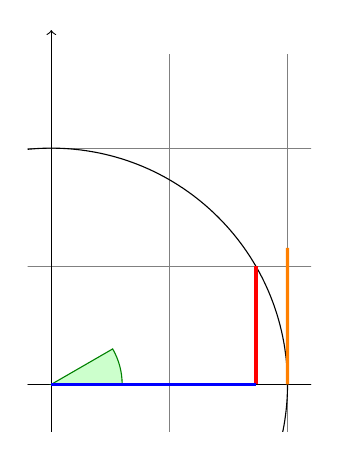
\begin{tikzpicture}[scale=3][>=latex']
    \clip (-0.1,-0.2) rectangle (1.1,1.51);
    \draw[step=.5cm,gray,very thin] (-1.4,-1.4) grid (1.4,1.4);
    \draw[->] (-1.5,0) -- (1.5,0);
    \draw[->] (0,-1.5) -- (0,1.5);
    \draw (0,0) circle [radius=1cm];
    \filldraw[fill=green!20,draw=green!50!black] (0,0) -- (3mm,0mm)
    arc [start angle=0, end angle=30, radius=3mm] -- cycle;
    \draw[red,very thick] (30:1cm) -- +(0,-0.5);
    \draw[blue,very thick] (30:1cm) ++(0,-0.5) -- (0,0);
    \path [name path=upward line] (1,0) -- (1,1);
    \path [name path=sloped line] (0,0) -- (30:1.5cm);
    \draw [name intersections={of=upward line and sloped line, by=x}]   % <-- Here
    [very thick,orange] (1,0) -- (x);
\end{tikzpicture}

\end{document}
